\documentclass[tikz,border=4pt]{standalone}
% Estilo común de los diagramas de bloques (se usa con \input en cada standalone)
\usepackage[defaultsans,scale=0.92]{lato}
\usepackage{libertinust1math}
\usepackage{xcolor,amsmath}
\usepackage{tikz}
\usetikzlibrary{positioning,arrows.meta,calc,shapes.geometric}
\usepackage{../../notacion}
\definecolor{ctrlazul}{HTML}{1E5AA8}\definecolor{ctrlnoche}{HTML}{14213D}
\definecolor{ctrlcoral}{HTML}{D1495B}\definecolor{ctrlverde}{HTML}{2A9D8F}
\definecolor{ctrlambar}{HTML}{E09F3E}\definecolor{ctrlgris}{HTML}{5C677D}
\definecolor{ctrlvioleta}{HTML}{6C4AB6}\definecolor{ctrlteal}{HTML}{0F7173}
\tikzset{
  >={Stealth[length=2.4mm]}, every node/.style={font=\small},
  bloque/.style={draw=ctrlnoche,fill=ctrlazul!7,thick,rounded corners=1.5pt,minimum height=9mm,minimum width=13mm,inner sep=4pt},
  suma/.style={draw=ctrlnoche,thick,circle,inner sep=0pt,minimum size=6mm},
  senal/.style={->,thick,draw=ctrlnoche},
  rot/.style={font=\footnotesize,text=ctrlgris},
}

\begin{document}
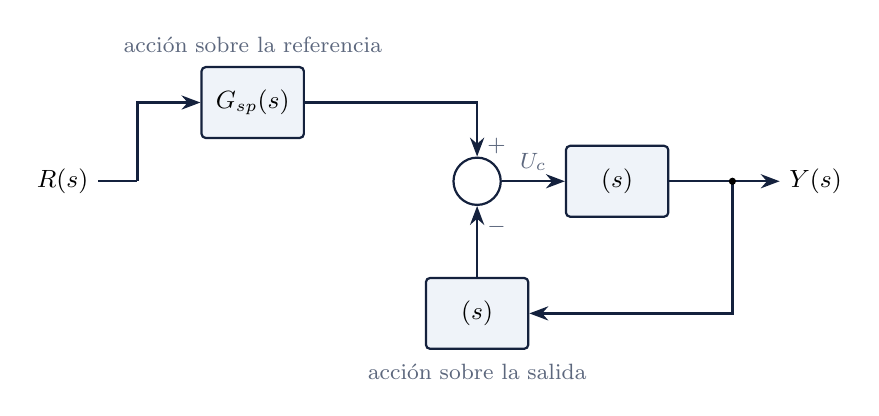
\begin{tikzpicture}
  \node (r) {$R(s)$};
  \coordinate[right=5mm of r] (r0);
  \node[bloque,right=8mm of r0,yshift=10mm] (Gsp) {$G_{sp}(s)$};
  \node[suma,right=40mm of r0] (S) {};
  \node[bloque,right=8mm of S] (P) {$\Gp(s)$};
  \coordinate[right=8mm of P] (y0);
  \node[right=6mm of y0] (y) {$Y(s)$};
  \node[bloque,below=9mm of S] (Gc) {$\Gc(s)$};
  \draw[thick,draw=ctrlnoche] (r) -- (r0);
  \draw[senal] (r0) |- (Gsp);
  \draw[senal] (Gsp) -| node[pos=0.9,right,rot]{$+$} (S);
  \draw[senal] (S) -- node[above,rot]{$U_c$} (P);
  \draw[senal] (P) -- (y);
  \draw[senal] (y0) |- (Gc);
  \draw[senal] (Gc) -- node[pos=0.7,right,rot]{$-$} (S);
  \fill (y0) circle (1.3pt);
  \node[rot,above=0.5mm of Gsp] {acción sobre la referencia};
  \node[rot,below=0.5mm of Gc] {acción sobre la salida};
\end{tikzpicture}
\end{document}
